%Goals
% You can use std::array and std::vector in your code
% You can use an iterator to access container elements
% You can access and modify container contents using algorithms
% You can interact with streams through iterators

\section{Sequences and Iterators}
\subsection{Introduction to std::array<T, N> and std::vector<T>}
\textbf{Array}\\
C++'s std::array<T, N> is a fixed-size Container.  T is a template type parameter (= placeholder for type). N is a positive integer, template non-type parameter (= placeholder for a value). Elements can be accessed with a subscript operator [] or at(). . The size is bound to the array object and can be queried using .size();. Avoid plain C-Array whenever possible: int arr[]{1, 2, 3, 4, 5};
\begin{itemize}
  \itemsep -0.5em 
  \item at() throws an exception on invalid index access
  \item $[]$ has undefined behavior on invalid index access Behavior
  \item The size of an array must be known at compile-time and cannot be changed. Otherwise it contains N default-constructed elements: std::array<int, 5> emptyArray{};
\end{itemize}
\begin{center}
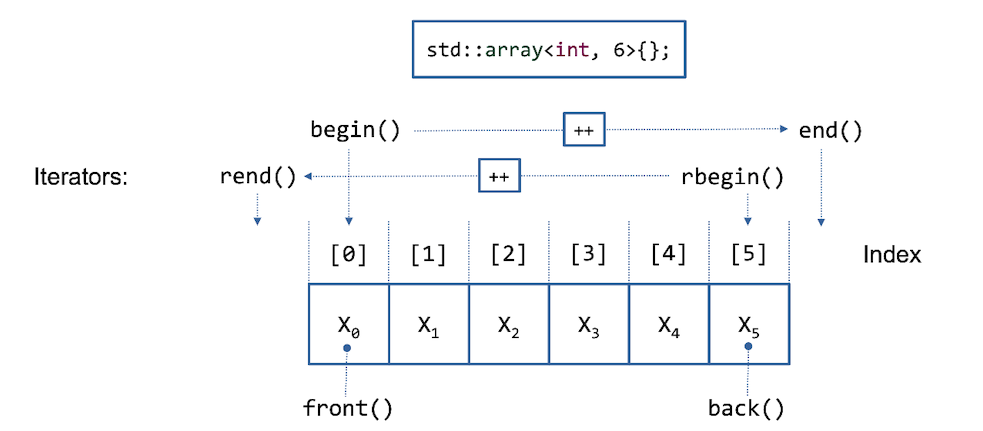
\includegraphics[width=0.75\linewidth]{images/array}
\end{center}

\textbf{Vector}\\
C++'s std::vector<T> is a Container = contains its elements of type T (no need to allocate them). java.util.ArrayList<T> is a collection = keeps references to T objects (must be “new”ed).  T is a template type parameter (= placeholder for type). std::vector can be initialized with a list of elements. Otherwise it is empty: std::vector<double> vd{};.
\begin{center}
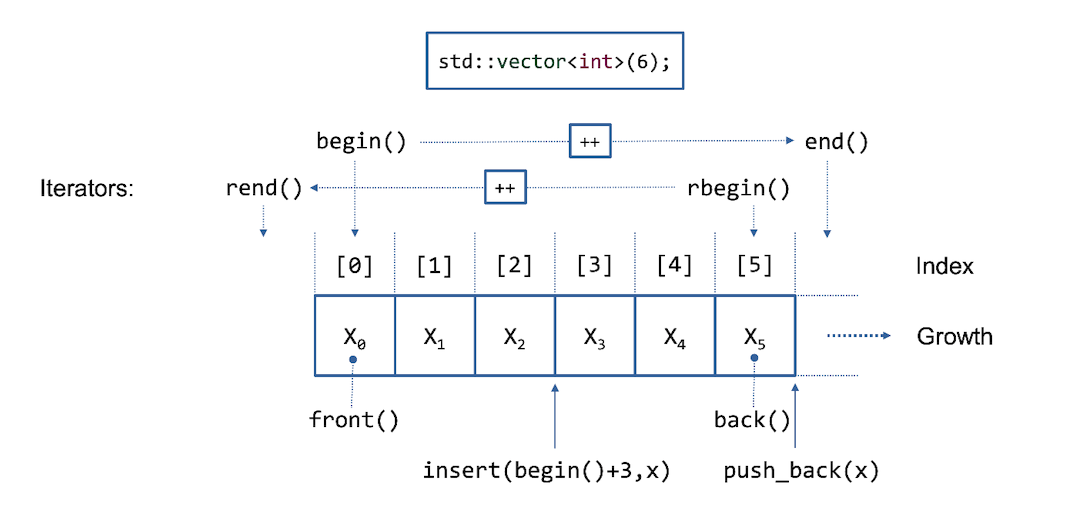
\includegraphics[width=0.75\linewidth]{images/vector}
\end{center}
\textbf{Append Elements to an std::vector<T>}
\begin{itemize}
  \itemsep -0.5em 
  \item $v.push\_back(<value>);$
  \item $v.insert (<iterator-position>, <value>);$
\end{itemize}

\textbf{Filling a Vector with Values}
\begin{lstlisting}[language=C++]
std::vecor<int> v{};
v.resize(10);
std::fill(std::begin(v), std::end(v), 2);

std::vector<int> v(10); 
std::fill(std::begin(v), std::end(v), 2);

std::vector v(10, 2);

// Filling increased values with iota
std::vector<int> v(100); std:iota(std::begin(v), std::end(v), 1);
\end{lstlisting}

\textbf{Finding and counting elements of a vector} \\
 std::find() and std::find\_if() return an iterator to the first element that matches the value or condition.
\begin{lstlisting}[language=C++]
auto zero_it = std::find(std::begin(v), std::end(v), 0); if (zero_it == std::end(v)) {
std::cout << "no zero found \n"; }
	
\end{lstlisting}



\subsection{Iteration}
Its possible to index a vector like an array but there is no bounds check.    Accessing an element outside the valid range is Undefined Behavior.

\textbf{Bad Style Iteration!}\\
\begin{lstlisting}[language=C++]
for (size_t i = 0; i < v.size(); ++i) {  //Index is "unsigned" 0-1=MAX_INT
	std::cout << "v[" << i << "] = " << v[i] << '\n'; }
}	
\end{lstlisting}

\textbf{Elemt Iteration (Range-Based for)}
\begin{itemize}
  \itemsep -0.5em 
  \item Advantage: No index error possible 
  \item Works with all containers, even value lists {1, 2, 3}
\end{itemize}

\begin{center}
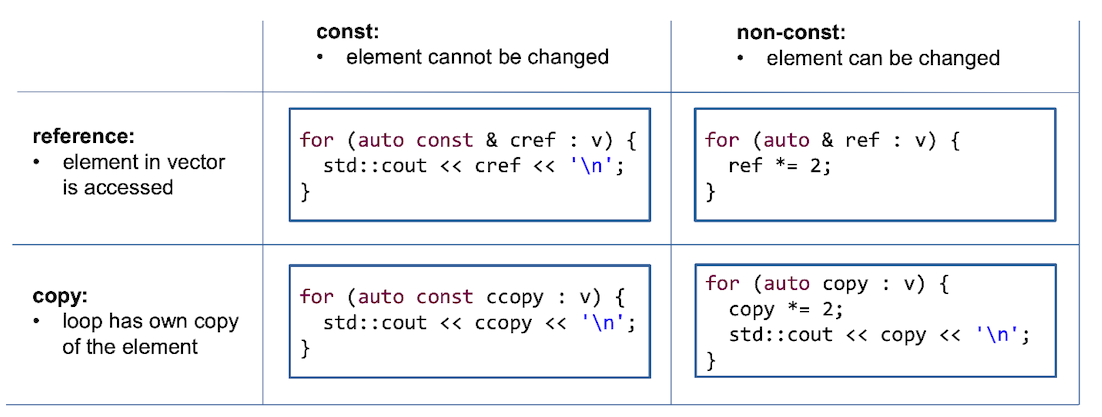
\includegraphics[width=0.75\linewidth]{images/elementiteration}	
\end{center}

\textbf{Iteration with Iterators}
\begin{lstlisting}[language=C++]
for (auto it = std::begin(v); it != std::end(v); ++it) {
	std::cout << (*it)++ << ", "; 
}
// Guarantee to just have read-only access with std::cbegin() and std::cend()
for (auto it = std::cbegin(v); it != std::cend(v); ++it) {
	std::cout << *it << ", "; 
}
\end{lstlisting}

\subsection{Using Iterators with Algorithms}
 Each algorithm takes iterator arguments. The algorithm does what its name tells us. 
 
\begin{lstlisting}[language=C++]
// Counting blanks in a string
size_t count_blanks(std::string s) {
 	size_t count{0};
 	for (size_t = 0; i < s.size(); ++i) {
 		if (s[i] == ' ') {
 			++count;
 		}
 	}
 	return count;
 }
 
// Counting blanks in a string with algorithms
size_t count_blanks(std::string s) {
	return std::count(s.begin(), s.end(), ' ');
}

// Summing up all values in a vector
std::vector<int> v{5, 4, 3, 2, 1}; 
std::cout << std::accumulate(std::begin(v), std::end(v), 0)<< " = sum\n";

// Number of elements in range 
void printDistanceAndLength(std::string s) {
	std::cout << "distance: "<< std::distance(s.begin(), s.end()) <<'\n';
	std::cout << "in a string of length: "<< s.size()<<'\n'; 
} 	

// Printing all values of a vector
void printAll(std::vector<int> v) {
	std::for_each(std::crbegin(v), std::crend(v), print); 
}

// For each with a Lambda
void printAll(std::vector<int> v, std::ostream & out) {
	std::for_each(std::crbegin(v), std::crend(v), [&out](auto x) {
		out << "print: "<< x << '\n';
	});
}

\end{lstlisting}


\subsection{Iterators for I/O}
Iterators connect streams and algorithms.  Streams (std::istream and std::ostream) cannot be used with algorithms directly.
\begin{itemize}
	\itemsep -0.5em 
  	\item $std::ostream\_iterator<T>$ outputs values of type T to the given std::ostream
  	\begin{itemize}
  		\item No end() marker needed for output, it ends when the input range ends.
  	\end{itemize}
  	
  	\item  $std::istream_iterator<T>$ reads values of type T from the given std::istream
	\begin{itemize}
  		\item End iterator is the default constructed $std::istream_iterator<T>{}$
   		\item It ends when the stream is no longer good().
   	\end{itemize}
\end{itemize}

\break